\documentclass{article}

% Anonymous NeurIPS 2026 submission.  Add [final] only after acceptance.
\usepackage{neurips_2026}
\usepackage[utf8]{inputenc}
\usepackage[T1]{fontenc}
\usepackage{hyperref}
\usepackage{url}
\usepackage{booktabs}
\usepackage{amsmath,amsfonts,amssymb}
\usepackage{microtype}
\usepackage{xcolor}
\usepackage{graphicx}
\usepackage{multirow}
\usepackage{array}
\usepackage{enumitem}
\usepackage{tikz}
\usetikzlibrary{arrows.meta,positioning,fit,shapes.geometric}

\newcommand{\method}{\textsc{LEGR-2Stage}}
\newcommand{\sbert}{\textsc{SBERT-FT}}
\newcommand{\vthree}{\textsc{LEGR-V3}}
\newcommand{\gps}{\textsc{LEGR-GPS}}
\newcommand{\Rone}{R@1}
\newcommand{\Rthree}{R@3}
\newcommand{\Rfive}{R@5}
\newcommand{\toolF}{Tool-F1}
\newcommand{\twR}{Twin-R@1}

\title{Beyond Tool Sets: Semantic Selection and Structural Reranking\\
for Twin-Aware Execution-Graph Retrieval}

\author{Anonymous Author(s)}

\begin{document}
\maketitle

\begin{abstract}
Retrieving an executable tool workflow from language requires two different decisions: which tools are needed, and how those tools depend on one another.
Standard dense retrieval benchmarks often make the first decision sufficient because each tool set occurs in only one candidate graph.
We show that this protocol can overstate structural planning ability: a fine-tuned Sentence-BERT model reaches 0.9267 Recall@1 on a compact 50-graph gallery, yet falls to 0.2133 when 272 same-tool-set structural alternatives are added.
We introduce a twin-aware evaluation protocol and a factorized architecture, \method, in which a frozen semantic expert selects the tool set and a frozen directed graph encoder plus a small residual pair scorer ranks only graphs in that set.
The reranker is trained exclusively from existing same-tool-set alternatives; no examples, labels, or splits are added or modified.
Across 15-, 30-, and 45-tool twin-filled galleries, the three-seed mean Recall@1 of \method{} is 0.2756, 0.3246, and 0.3611, versus 0.2133, 0.1762, and 0.1700 for \sbert{}, while tool-set F1 is preserved exactly.
The 15-tool gain is post-hoc and inconclusive with 50 DAG clusters, whereas the architecture-fixed 30- and 45-tool gains are significant under DAG-clustered paired bootstrap (95\% CIs $[0.0563,0.2405]$ and $[0.1244,0.2589]$).
A separately trained V3 is strongest at 45 tools (0.4183 Recall@1), revealing a scale-dependent tradeoff between unconstrained structural ranking and guaranteed semantic preservation.
A 65-run architecture search further shows that a query-gated GPS model wins on the original development gallery but fails on the twin-filled evaluation, demonstrating the importance of matching model selection to the intended structural test.
Finally, a representation audit finds significant organization by dominant read, edit, and orchestration function (5-NN macro-F1 0.9462, permutation $p\leq0.001$), connecting functional tool semantics to graph-level geometry without treating visualization as evidence.
\end{abstract}

\section{Introduction}

Tool-augmented language models must map an instruction to both a set of operations and an executable dependency structure \cite{schick2023toolformer,patil2023gorilla,qin2023toolllm,shen2023hugginggpt}.
These requirements are easy to conflate.
If a benchmark contains only one graph for each tool set, a model can retrieve the correct graph by recognizing tool names while ignoring edge direction, parallelism, and reachability.
This shortcut is especially attractive to pretrained text encoders: a serialized workflow contains rich lexical information even when its graph structure is represented weakly.

We study this problem through \emph{structural twins}: candidate DAGs that use exactly the same multiset of tools but differ in their directed edges.
Twins transform graph retrieval from semantic set matching into the decision a workflow planner actually faces: whether operations form a chain, a fork, a join, or a partially ordered composition.
Our Campaign-v4 evaluation combines 50 held-out gold DAGs with 272 candidate-only structural alternatives.
All 300 held-out queries are twin eligible, and the resulting 322-graph gallery contains 927 same-tool-set graph pairs.

This evaluation changes the empirical conclusion.
On the compact 50-DAG gallery, \sbert{} obtains 0.9267 Recall@1 and \vthree{} obtains 0.8267.
On the twin-filled gallery, both fall near 0.21, and \vthree{} has only a small advantage on same-tool-set ranking (0.2367 versus 0.2333).
A broad 65-run model-only search produces \gps{}, a directed GPS adapter with query-conditioned semantic fusion.
It improves development Recall@1 from 0.8742 to 0.9138, but its three-seed mean is only 0.1333 on the twin-filled gallery.
The apparent development win did not transfer because the selection gallery contained only five two-DAG twin groups.

The failure suggests a simple mathematical decomposition.
Tool-set prediction is already strong; unconstrained fusion allows a noisy structural score to damage it.
We therefore make semantics a hard first-stage constraint rather than a soft expert.
\sbert{} chooses a tool set, after which a V3-initialized pair scorer ranks only candidates sharing that set.
This design preserves semantic accuracy by construction and spends the learned capacity solely on edge-order discrimination.

Our contributions are:
\begin{itemize}[leftmargin=*]
    \item We expose a \textbf{tool-set shortcut} in execution-graph retrieval and introduce a deterministic, tie-aware 322-DAG evaluation in which every held-out query has same-tool-set alternatives.
    \item We propose \textbf{\method{}}, a factorized semantic-selection/structural-reranking architecture.  Only a 264,705-parameter residual pair head is trained after tier-specific \sbert{} and \vthree{} training.
    \item We report the complete path to the result, including a 65-run objective, encoder, readout, fusion, reranking, and optimization search whose development winner fails on the harder gallery.  This negative result motivates the final factorization.
    \item We confirm the fixed architecture at 30 and 45 tools, report paired uncertainty, and compare against corrected GPT-OSS 120B and Llama 3.2 DAG generators without conflating single-output exact match with retrieval Recall@k.
    \item We connect functional categorization to learned representation geometry through an original-space clustering audit, while carefully distinguishing corroboration from causal or zero-shot evidence.
\end{itemize}

\section{Related Work}

\paragraph{Tool use and workflow planning.}
Toolformer, Gorilla, ToolBench, BFCL, and related systems study the selection and invocation of external tools \cite{schick2023toolformer,patil2023gorilla,qin2023toolllm,yan2024berkeley}.
ReAct and plan-then-execute approaches generate intermediate reasoning or action sequences autoregressively \cite{yao2023react,wang2023plan}.
Retrieval offers a complementary operating point: candidates can be validated offline, graph embeddings can be cached, and inference need not generate a plan token by token.

\paragraph{Dense and graph retrieval.}
Sentence-BERT provides an efficient dual-encoder baseline for semantic retrieval \cite{reimers-gurevych-2019-sentence}; MiniLM supplies the compact shared language backbone used here \cite{wang2020minilm}.
Graph neural networks aggregate local structure \cite{kipf2017semi,hamilton2017inductive,velickovic2018graph,xu2018how}, while Graphormer and GPS-style models augment local propagation with global, relation-biased attention \cite{ying2021transformers,rampasek2022recipe}.
Our main conclusion is not that one graph operator is universally superior, but that the retrieval objective and candidate gallery must force the model to use graph structure.

\paragraph{Hard negatives and graph similarity.}
Contrastive learning depends critically on the negative distribution \cite{oord2018representation,chen2020simple,you2020graph}.
Graph edit distance (GED) is a natural structural dissimilarity measure \cite{sanfeliu1983distance,abu2015exact}, but our ablations show that GED regularization is not uniformly beneficial.
Same-tool-set twins are more direct negatives for the retrieval decision: lexical content is held approximately fixed while edge structure changes.

\section{Problem Formulation}

Let $q$ be a natural-language request and let $\mathcal{C}=\{G_j\}_{j=1}^{M}$ be a gallery of validated execution DAGs.
A graph $G=(V,E)$ has tool-labeled nodes and directed dependency edges.
Let $T(G)$ denote its canonical tool multiset.
Exact-plan retrieval predicts
\begin{equation}
    \hat G(q)=\arg\max_{G\in\mathcal C}s(q,G).
\end{equation}
We report Recall@$k$, MRR@5, and mean GED error.
Tool-set F1 compares $T(\hat G)$ with $T(G^+)$, separating semantic tool choice from exact structure.

For each gold graph $G^+$, define its twin set
\begin{equation}
    \mathcal N_{\mathrm{twin}}(G^+)=
    \{G\in\mathcal C:T(G)=T(G^+),\;G\not\cong G^+\}.
\end{equation}
A query is twin eligible when this set is nonempty.
We report \twR{} and pairwise accuracy against every member of $\mathcal N_{\mathrm{twin}}$.
Unlike ordinary Recall@1, these metrics cannot be solved by choosing the correct tool set alone.

We compute both stable-order metrics and the expected metric under uniform breaking of score ties within $10^{-5}$; tables report the stable-order value for continuity, and complete artifacts include both.
Candidate order is obtained by sorting canonical graph keys and applying a seeded permutation.
For the reported models, tie-aware Recall@1 differs by at most 0.0017 and does not change a conclusion.
This audit exposes an artifact in tools-only serialization: because twin strings become identical, conventional first-index tie breaking can move restricted Recall@1 from 0 to 0.9733 without changing a single score.

\section{Models}

\subsection{Semantic and structural experts}

\paragraph{\sbert.}
The semantic expert is an existing fine-tuned Sentence-BERT dual encoder.
It embeds the query and a serialized candidate plan with a shared MiniLM backbone and uses cosine similarity $s_S(q,G)$.
Throughout this paper, ``\sbert{}'' and the frozen semantic expert refer to the same trained checkpoint; we avoid introducing a separate ``control'' model name.

\paragraph{\vthree.}
The structural expert initializes each tool node from the shared MiniLM text encoder, performs directed message passing with separate incoming and outgoing transformations, and combines a node-set representation with a graph representation.
It produces normalized query and graph vectors $z_q,z_G\in\mathbb R^{256}$ and cosine score
\begin{equation}
    s_V(q,G)=z_q^\top z_G.
\end{equation}
V3's graph-dependent embedding separates twins that tools-only text collapses, but its semantic tool selection remains weaker than \sbert{}.

\subsection{A failed soft-fusion route: \gps}

Our first research architecture adds four layers of directed local propagation and relation-biased global attention, degree/source/sink structural features, dual-attention pooling, tool-membership and five-way relation heads, and a query-conditioned mixture over five scores.
The relation labels are parallel, direct forward, indirect forward, direct reverse, and indirect reverse.
This architecture is useful diagnostically: it wins on the original development gallery but fails to transfer to the twin-filled gallery (Section~\ref{sec:results}).
Its failure motivates hard factorization.

\subsection{Proposed two-stage structural reranker}

\begin{figure}[t]
\centering
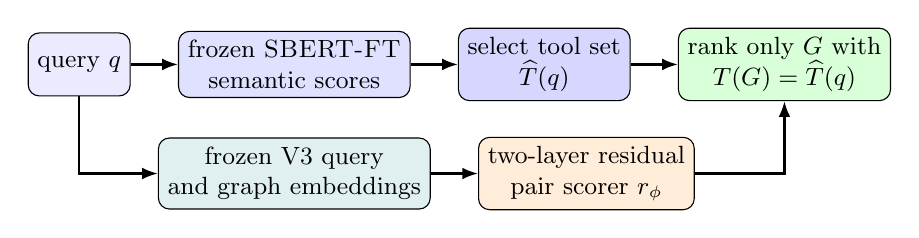
\begin{tikzpicture}[
  node distance=5mm and 6mm,
  box/.style={draw,rounded corners,align=center,minimum height=8mm,font=\small},
  arr/.style={-{Latex[length=2mm]},thick}
]
\node[box,fill=blue!8] (q) {query $q$};
\node[box,fill=blue!12,right=of q] (sbert) {frozen \sbert\\semantic scores};
\node[box,fill=blue!16,right=of sbert] (set) {select tool set\\$\widehat T(q)$};
\node[box,fill=teal!12,below=of sbert] (v3) {frozen V3 query\\and graph embeddings};
\node[box,fill=orange!15,right=of v3] (head) {two-layer residual\\pair scorer $r_\phi$};
\node[box,fill=green!15,right=of set] (rank) {rank only $G$ with\\$T(G)=\widehat T(q)$};
\draw[arr] (q)--(sbert);
\draw[arr] (sbert)--(set);
\draw[arr] (q)|-(v3);
\draw[arr] (v3)--(head);
\draw[arr] (set)--(rank);
\draw[arr] (head)-|(rank);
\end{tikzpicture}
\caption{\textbf{\method{}.}  Semantic selection is a hard constraint, not a learned mixture.  \sbert{} selects the exact tool set; a V3-initialized pair scorer ranks only structural twins in that set.  Both experts are frozen.}
\label{fig:twostage}
\end{figure}

The first stage selects the tool set of \sbert{}'s top candidate:
\begin{equation}
    \widehat T(q)=T\!\left(\arg\max_{G\in\mathcal C}s_S(q,G)\right).
    \label{eq:stage1}
\end{equation}
The second stage scores only $\mathcal C_{\widehat T}=\{G:T(G)=\widehat T(q)\}$.
From frozen V3 embeddings we construct a symmetric comparison feature
\begin{equation}
    u(q,G)=[z_q;z_G;|z_q-z_G|;z_q\odot z_G]\in\mathbb R^{1024}.
\end{equation}
A small MLP predicts a residual
\begin{equation}
    r_\phi(q,G)=w_2^\top\mathrm{Dropout}\!\left(
    \mathrm{GELU}(W_1\mathrm{LN}(u)+b_1)\right)+b_2,
\end{equation}
where $W_1\in\mathbb R^{256\times1024}$.
The structural score is
\begin{equation}
    s_\phi(q,G)=z_q^\top z_G+r_\phi(q,G),
\end{equation}
and prediction is
\begin{equation}
    \hat G(q)=\arg\max_{G\in\mathcal C_{\widehat T(q)}}s_\phi(q,G).
    \label{eq:stage2}
\end{equation}
We initialize $(w_2,b_2)$ to zero, so training begins exactly at the inherited V3 cosine score.
Only $\phi$ is updated, totaling 264,705 trainable parameters.

For query $q_i$, gold $G_i^+$, and a same-tool-set negative $G_{ij}^-$, we minimize pairwise softplus ranking:
\begin{equation}
    \mathcal L_{\mathrm{pair}}=
    \frac{1}{|\mathcal P|}\sum_{(i,j)\in\mathcal P}
    \log\left(1+\exp\left[s_\phi(q_i,G_{ij}^-)-s_\phi(q_i,G_i^+)\right]\right).
    \label{eq:pairloss}
\end{equation}
Training pairs are derived in memory from existing train graphs that share a tool set; no synthetic graph or query is introduced.
The hard constraint in Eq.~\ref{eq:stage2} makes the final tool-set prediction identical to Stage~1 by construction.

\section{Campaign-v4 Benchmark}

\subsection{Tools, graphs, and language}

Campaign-v4 contains an action-first registry of 45 tools in nested 15-, 30-, and 45-tool tiers.
At 15 tools there are six read/retrieval, six edit/modification, and three orchestration tools.
Graphs cover 20 training/development topology families; diamond and asymmetric fork--join families are excluded from both and used for topology-held-out testing.
Every DAG has six GPT-4o-generated query variants: standard, paraphrase, lexical, confusable, structurally clear, and structural paraphrase.

\begin{table}[t]
\caption{Campaign-v4 statistics.  Twin-filled evaluation is reported at every tier.}
\label{tab:data}
\centering
\small
\begin{tabular}{lrrrr}
\toprule
Tier / split & Rows & DAGs & Tool sets & Role \\
\midrule
15 / train & 1,488 & 248 & 159 & optimization \\
15 / dev & 294 & 49 & 44 & selection \\
15 / in-domain test & 192 & 32 & 30 & auxiliary \\
15 / topology held-out & 300 & 50 & 49 & gold queries \\
15 / candidate-only & 1,632 & 272 & 49 & structural twins \\
\midrule
30 / train, dev, held-out & 2,910 & 485 & -- & scale resource \\
45 / train, dev, held-out & 4,182 & 697 & -- & scale resource \\
\bottomrule
\end{tabular}
\end{table}

The 15-tool split contains no canonical-DAG overlap between train/development and topology-held-out test.
The candidate-only file does not contain held-out gold DAGs; it supplies alternatives and cannot be evaluated alone.
All protected datasets, original model sources, and existing checkpoints were hashed before and after experimentation.
The final integrity reports contain no changed, missing, or added protected files.

\subsection{Compact versus twin-aware galleries}

We distinguish two protocols.
The \emph{compact} gallery contains the 50 held-out gold DAGs, nearly one per tool set.
It primarily measures semantic matching.
The \emph{twin-filled} gallery is the union of those gold DAGs and 272 candidate-only graphs, totaling 322 candidates, 49 tool sets, and 927 twin pairs.
Every held-out query has at least one same-tool-set alternative.

For the two-stage follow-up, each development gallery is expanded with its tier's training DAGs: 297, 415, and 597 candidates at 15, 30, and 45 tools.
This does not move examples across splits: checkpoints are selected using the original development queries (294/414/594 by tier), while training DAGs act only as candidate distractors.
At 15 tools the expansion yields 150 twin-eligible development queries over 25 gold DAGs, compared with five two-DAG twin groups in the original gallery; the larger tiers yield 222 and 342 twin-eligible development queries.

\section{Experimental Protocol}

All search experiments use the existing MiniLM checkpoint available locally.
The broader search considered multi-positive InfoNCE, pairwise and listwise twin losses, tool membership, five-way relation prediction, reachability-distance regularization, group-aware sampling, directed residual/Gated/PNA-style/Graphormer/GPS encoders, five structural encodings, five readouts, semantic fusion, candidate-aware reranking, partial unfreezing, cosine/plateau schedules, EMA, SWA, online hard negatives, and a twin curriculum.
Alternative MPNet, E5, and BGE backbones were unavailable locally and were not downloaded.

The 65-run search used seed 42 for screening and seeds 42, 123, and 2026 for confirmation.
For scaling, one no-GED V3 checkpoint is trained at each tier with seed 42, a 75-epoch cap, and validation-loss early stopping, matching the established V3 protocol.
The final two-stage reranker uses seeds 42, 123, and 2026 at every tier and selects checkpoints by lexicographic development performance: structural twin Recall@1, end-to-end Recall@1, then hard-negative pair accuracy.
Each tier evaluator uses a fixed candidate permutation, expected metrics under score ties, and 10,000 paired bootstrap replicates clustered by canonical gold DAG so that six paraphrases are resampled together.

The original locked evaluation of \sbert{}, V3, and GPS preceded the two-stage proposal.
Consequently, \method{}'s 322-DAG result is a \emph{post-hoc exploratory follow-up}, not pristine confirmatory evidence.
We make this chronology explicit rather than relabeling the already inspected gallery as a new test set.

\section{Results}
\label{sec:results}

\subsection{Compact evaluation masks the structural problem}

\begin{table}[t]
\caption{The compact gallery rewards tool semantics; adding same-tool-set alternatives changes the ranking problem.}
\label{tab:protocolshift}
\centering
\small
\begin{tabular}{lrrrr}
\toprule
Model & Gallery & \Rone{} & \toolF{} & \twR{} \\
\midrule
\sbert{} & 50 compact & 0.9267 & 0.9811 & -- \\
\vthree{} & 50 compact & 0.8267 & 0.9464 & -- \\
\midrule
\sbert{} & 322 twin-filled & 0.2133 & 0.9689 & 0.2333 \\
\vthree{} & 322 twin-filled & 0.2100 & 0.9508 & 0.2367 \\
\bottomrule
\end{tabular}
\end{table}

Table~\ref{tab:protocolshift} demonstrates the shortcut directly.
The 71.3-point decline for \sbert{} is not a degradation of its checkpoint; the queries are identical, but the gallery now contains structurally different graphs with nearly indistinguishable lexical content.
V3's small Twin-R@1 advantage suggests useful structural signal, while SBERT retains the stronger tool-set decision.
This complementarity motivates Eqs.~\ref{eq:stage1}--\ref{eq:stage2}.

\subsection{The soft-fusion development winner does not transfer}

The three-seed \gps{} confirmation reaches development Recall@1 $0.9138\pm0.0098$ and tool-set F1 $0.9883\pm0.0008$, compared with 0.8742 and 0.9809 for the frozen \sbert{} expert in the same evaluation code.
On the twin-filled held-out evaluation, however, its mean Recall@1 is 0.1333 and Twin-R@1 is 0.1444.
The paired Recall@1 difference from \sbert{} is $-0.0800$ with a DAG-clustered 95\% CI of $[-0.1378,-0.0211]$.
The negative result is statistically clear: the learned gate selected on an easy gallery did not learn a transferable division of semantic and structural responsibility.

\subsection{Two-stage factorization improves the point estimate}

\begin{table*}[t]
\caption{Main 322-DAG twin-filled results.  Mean$\pm$sample SD is over three seeds.  All 300 queries are twin eligible.  \method{} preserves \sbert{}'s tool set exactly by construction.}
\label{tab:main}
\centering
\small
\begin{tabular}{lrrrrrrr}
\toprule
Model & \Rone{} & \Rthree{} & \Rfive{} & MRR@5 & \toolF{} & \twR{} & Pair acc. \\
\midrule
\sbert{} & 0.2133 & 0.6100 & 0.8533 & 0.4359 & 0.9689 & 0.2333 & 0.6687 \\
\vthree{} & 0.2100 & 0.5667 & 0.8133 & 0.4239 & 0.9508 & 0.2367 & 0.6960 \\
\gps{} (3-seed mean) & 0.1333 & 0.5700 & 0.7922 & 0.3633 & 0.9668 & 0.1444 & 0.6135 \\
\midrule
\method{}, seed 42 & 0.2767 & 0.6833 & 0.8800 & 0.5023 & 0.9689 & 0.2767 & 0.6882 \\
\method{}, seed 123 & 0.2633 & 0.6333 & 0.8767 & 0.4865 & 0.9689 & 0.2633 & 0.6698 \\
\method{}, seed 2026 & \textbf{0.2867} & \textbf{0.6900} & 0.8800 & \textbf{0.5069} & 0.9689 & \textbf{0.2867} & 0.6911 \\
\method{} mean & \textbf{0.2756}$\pm$.0117 & \textbf{0.6689}$\pm$.0310 & \textbf{0.8789}$\pm$.0019 & \textbf{0.4986}$\pm$.0107 & \textbf{0.9689}$\pm$.0000 & \textbf{0.2756}$\pm$.0117 & \textbf{0.6830}$\pm$.0115 \\
\bottomrule
\end{tabular}
\end{table*}

\method{} improves the mean exact Recall@1 by 0.0622 (29.2\% relative) and Twin-R@1 by 0.0422 over \sbert{}, while preserving tool-set F1 exactly.
All three seeds improve Recall@1, with a narrow seed range of 0.2633--0.2867.
The factorization also improves R@3, R@5, and MRR@5.

The paired uncertainty, however, remains wide because the effective independent sample is 50 DAGs rather than 300 paraphrases.
The DAG-clustered 95\% CI is $[-0.0356,0.1644]$ for Recall@1 and $[-0.0589,0.1467]$ for Twin-R@1.
Tool-set F1 has a point difference and interval of exactly zero.
Thus the result is a reproducible point-estimate improvement, not evidence that satisfies a predeclared confidence-interval-excludes-zero win criterion.

\subsection{Hard-development selection}

On the 297-DAG development gallery, \sbert{} obtains 0.5782 Recall@1 and 0.4333 Twin-R@1.
The two-stage seeds obtain 0.7551--0.7585 Recall@1 and 0.7267--0.7333 Twin-R@1.
The structural scorer alone reaches 0.8200--0.8267 Twin-R@1 when evaluated with the gold tool set.
The large development margin and smaller held-out margin indicate that the reranker learns training-family edge distinctions but only partially transfers to held-out diamond and asymmetric fork--join topologies.

\subsection{Scaling to 30 and 45 tools}

We next fix the architecture and train tier-specific V3 checkpoints on the existing 30- and 45-tool training splits.
Their checkpoints are selected on the corresponding development splits; the held-out galleries are not used for model or epoch selection.
The fair galleries contain 455 candidates/420 queries at 30 tools and 650 candidates/600 queries at 45 tools, and every query is twin eligible.

\begin{table*}[t]
\caption{Scaling on twin-filled held-out galleries. Two-stage values are mean$\pm$sample SD over three reranker seeds; SBERT-FT and V3 use the fixed seed-42 tier checkpoint. Bold marks the highest exact R@1 per tier.}
\label{tab:scaling}
\centering
\small
\begin{tabular}{rrlrrrrrr}
\toprule
Tools & Gallery & Model & \Rone{} & \Rthree{} & \Rfive{} & MRR@5 & \toolF{} & \twR{} \\
\midrule
15 & 322 & \sbert{} & .2133 & .6100 & .8533 & .4359 & .9689 & .2333 \\
   &     & \vthree{} & .2100 & .5667 & .8133 & .4239 & .9508 & .2367 \\
   &     & \method{} & \textbf{.2756}$\pm$.0117 & .6689 & .8789 & .4986 & .9689 & .2756 \\
\midrule
30 & 455 & \sbert{} & .1762 & .6000 & .9119 & .4198 & .9747 & .1762 \\
   &     & \vthree{} & .2310 & .7524 & .8976 & .4969 & .9737 & .2357 \\
   &     & \method{} & \textbf{.3246}$\pm$.0144 & .8198 & .9524 & .5714 & .9747 & .3246 \\
\midrule
45 & 650 & \sbert{} & .1700 & .6500 & .8883 & .4276 & .9747 & .1767 \\
   &     & \vthree{} & \textbf{.4183} & .8167 & .9400 & \textbf{.6239} & .9711 & \textbf{.4333} \\
   &     & \method{} & .3611$\pm$.0347 & .8167 & \textbf{.9467} & .5934 & \textbf{.9747} & .3611 \\
\bottomrule
\end{tabular}
\end{table*}

The two-stage improvement over \sbert{} grows with tool count: $+0.0622$, $+0.1484$, and $+0.1911$ Recall@1 at 15, 30, and 45 tools.
The 30-tool DAG-clustered 95\% CI is $[0.0563,0.2405]$ and the 45-tool interval is $[0.1244,0.2589]$, both excluding zero; the corresponding Twin-R@1 intervals are $[0.0536,0.2377]$ and $[0.1183,0.2483]$.
In contrast, the 15-tool interval crosses zero.
Because the architecture was fixed from the 15-tool study before these runs, the larger tiers provide stronger cross-tier evidence than the post-hoc 15-tool result.

The 45-tool row also qualifies the architectural claim: standalone V3 reaches the best exact score, 0.4183, and Twin-R@1, 0.4333.
Its tool-set F1 is 0.9711 rather than SBERT-FT's 0.9747.
Thus hard factorization provides a guarantee---exactly preserving the semantic expert's tool set---but can discard correct V3 predictions when the two experts disagree.
The result supports complementary operating points rather than universal dominance: use V3 when exact structure is primary, and \method{} when semantic tool-set preservation is a hard requirement.

\subsection{Comparison with DAG generators}

\begin{table}[t]
\caption{Corrected single-output DAG generation. Exact match (EM) is not retrieval Recall@1. Latency is wall-clock generation time.}
\label{tab:llm}
\centering
\scriptsize
\begin{tabular}{lrrrrrr}
\toprule
Model & Tools & $n$ & Tool-F1 & EM & Mean GED & mean/p95 s \\
\midrule
GPT-OSS 120B & 15 & 50 & .9450 & .76 & .44 & 3.05/4.47 \\
             & 30 & 50 & .9517 & .80 & .62 & 3.27/4.78 \\
             & 45 & 50 & .9486 & .76 & .80 & 3.11/4.61 \\
Llama 3.2 3B & 15 & 50 & .7911 & .08 & 6.11 & 4.49/15.30 \\
              & 30 & 50 & .7769 & .06 & 4.80 & 4.61/15.04 \\
              & 45 & 50 & .6844 & .04 & 4.58 & 5.08/15.69 \\
\bottomrule
\end{tabular}
\end{table}

GPT-OSS is a strong generator under its protocol, with 0.76--0.80 exact match and no parse failures or cycles in the corrected runs.
Llama has 0.04--0.08 exact match, 0--5 parse failures depending on tier, and 2--6 cyclic outputs.
These figures are not directly comparable to Table~\ref{tab:scaling}: a generator emits one potentially novel graph from a 50-query sample, whereas a retriever ranks a fixed 322--650-candidate gallery for all held-out queries.
We therefore compare their failure modes and resource profiles, not declare a winner from unlike columns.

\section{Ablations and Search Evidence}

\subsection{Objectives, sampling, and architecture}

\begin{table*}[t]
\caption{Representative seed-42 development screens from the 65-run search.  Stages are sequential rather than a full factorial ablation; bold identifies the best row within each displayed block.}
\label{tab:ablations}
\centering
\scriptsize
\begin{tabular}{llrrrr}
\toprule
Block & Variant & \Rone{} & \toolF{} & Toolset R@1 & p95 ms \\
\midrule
Objective & listwise only & 0.8980 & 0.9866 & 0.9388 & 2.11 \\
& + all auxiliary terms & 0.8912 & 0.9837 & 0.9456 & 1.54 \\
& pairwise twin, margin 0.2 & 0.9014 & 0.9862 & 0.9456 & 1.49 \\
& \textbf{auxiliary weights $\times0.5$} & \textbf{0.9048} & \textbf{0.9867} & 0.9456 & 1.51 \\
& random rather than group-aware batches & 0.8878 & 0.9780 & \textbf{0.9490} & 1.49 \\
\midrule
Encoder & residual directed / combined & 0.9048 & 0.9867 & 0.9456 & 1.55 \\
& Graphormer / none & 0.9116 & 0.9873 & 0.9490 & 13.63 \\
& GPS / combined & 0.9116 & 0.9878 & 0.9490 & 13.64 \\
& \textbf{GPS / degree-source-sink} & \textbf{0.9150} & \textbf{0.9892} & 0.9490 & 15.09 \\
& GPS / path mode & 0.9082 & 0.9873 & 0.9490 & 13.43 \\
\midrule
Readout & mean/V3-style & \textbf{0.9082} & 0.9872 & \textbf{0.9456} & 2.02 \\
& dual attention & 0.9048 & 0.9867 & \textbf{0.9456} & 1.92 \\
& virtual attention & \textbf{0.9082} & \textbf{0.9879} & \textbf{0.9456} & 1.63 \\
& Set2Set & 0.8912 & 0.9829 & 0.9388 & 1.45 \\
\bottomrule
\end{tabular}
\end{table*}

Several conclusions are robust enough to guide design.
First, stronger auxiliary losses do not monotonically improve exact retrieval; doubling their weight lowers development Recall@1 to 0.8673.
Second, group-aware batches are much faster and improve overall retrieval, although random batches slightly improve the restricted metric.
Third, global attention yields small gains on the original development gallery at roughly an order-of-magnitude greater cached-query latency.
Fourth, readout differences are minor and were not tested factorially on the final GPS encoder.

\subsection{Fusion is the pivotal ablation}

\begin{table}[t]
\caption{Fusion on the original 49-DAG development gallery.}
\label{tab:fusion}
\centering
\small
\begin{tabular}{lrrr}
\toprule
Fusion & \Rone{} & \toolF{} & Toolset R@1 \\
\midrule
GPS graph only & 0.8707 & 0.9708 & 0.9422 \\
\sbert{} only & 0.8742 & 0.9809 & 0.9320 \\
Fixed mean & 0.7211 & 0.8664 & 0.9456 \\
Learned scalar & 0.7211 & 0.8662 & 0.9456 \\
Query-conditioned gate & \textbf{0.9150} & \textbf{0.9892} & \textbf{0.9490} \\
\bottomrule
\end{tabular}
\end{table}

Naive fusion mixes incompatible score scales and fails sharply.
The query-conditioned gate appears to solve this problem on development, but Table~\ref{tab:main} shows that it does not generalize to the dense twin gallery.
Hard two-stage factorization removes scale calibration from the decision: semantics defines a feasible set; structure orders that set.

Candidate-aware cross-attention rerankers at $K\in\{10,20,40\}$ and one or two layers all stayed below 100 ms p95 but reduced development Recall@1 to 0.5884--0.7857 and tool F1 to 0.8318--0.9418.
Likewise, freezing the GPS backbone yielded 0.8571 Recall@1, while unfreezing the last two or all layers reached 0.9150; full unfreezing added latency without accuracy gain.
Cosine scheduling matched 0.9150; plateau, EMA, and SWA reached 0.9082; online hard negatives reached 0.9116; and twin curriculum preserved 0.9150 while producing the best restricted score, 0.9524.

\section{Functional Geometry}

Functional categorization groups tools by operational effect---read, edit, or orchestrate---rather than topic.
To test whether these labels are reflected in learned graph geometry, we deterministically label each graph by its uniquely dominant registry action category.
Exact ties are labeled mixed and excluded from the primary three-class audit.
Across all 651 unique 15-tool graphs, this yields 232 read, 223 edit, 32 orchestrate, and 164 mixed graphs; 487 enter the primary analysis.

\begin{figure}[t]
\centering
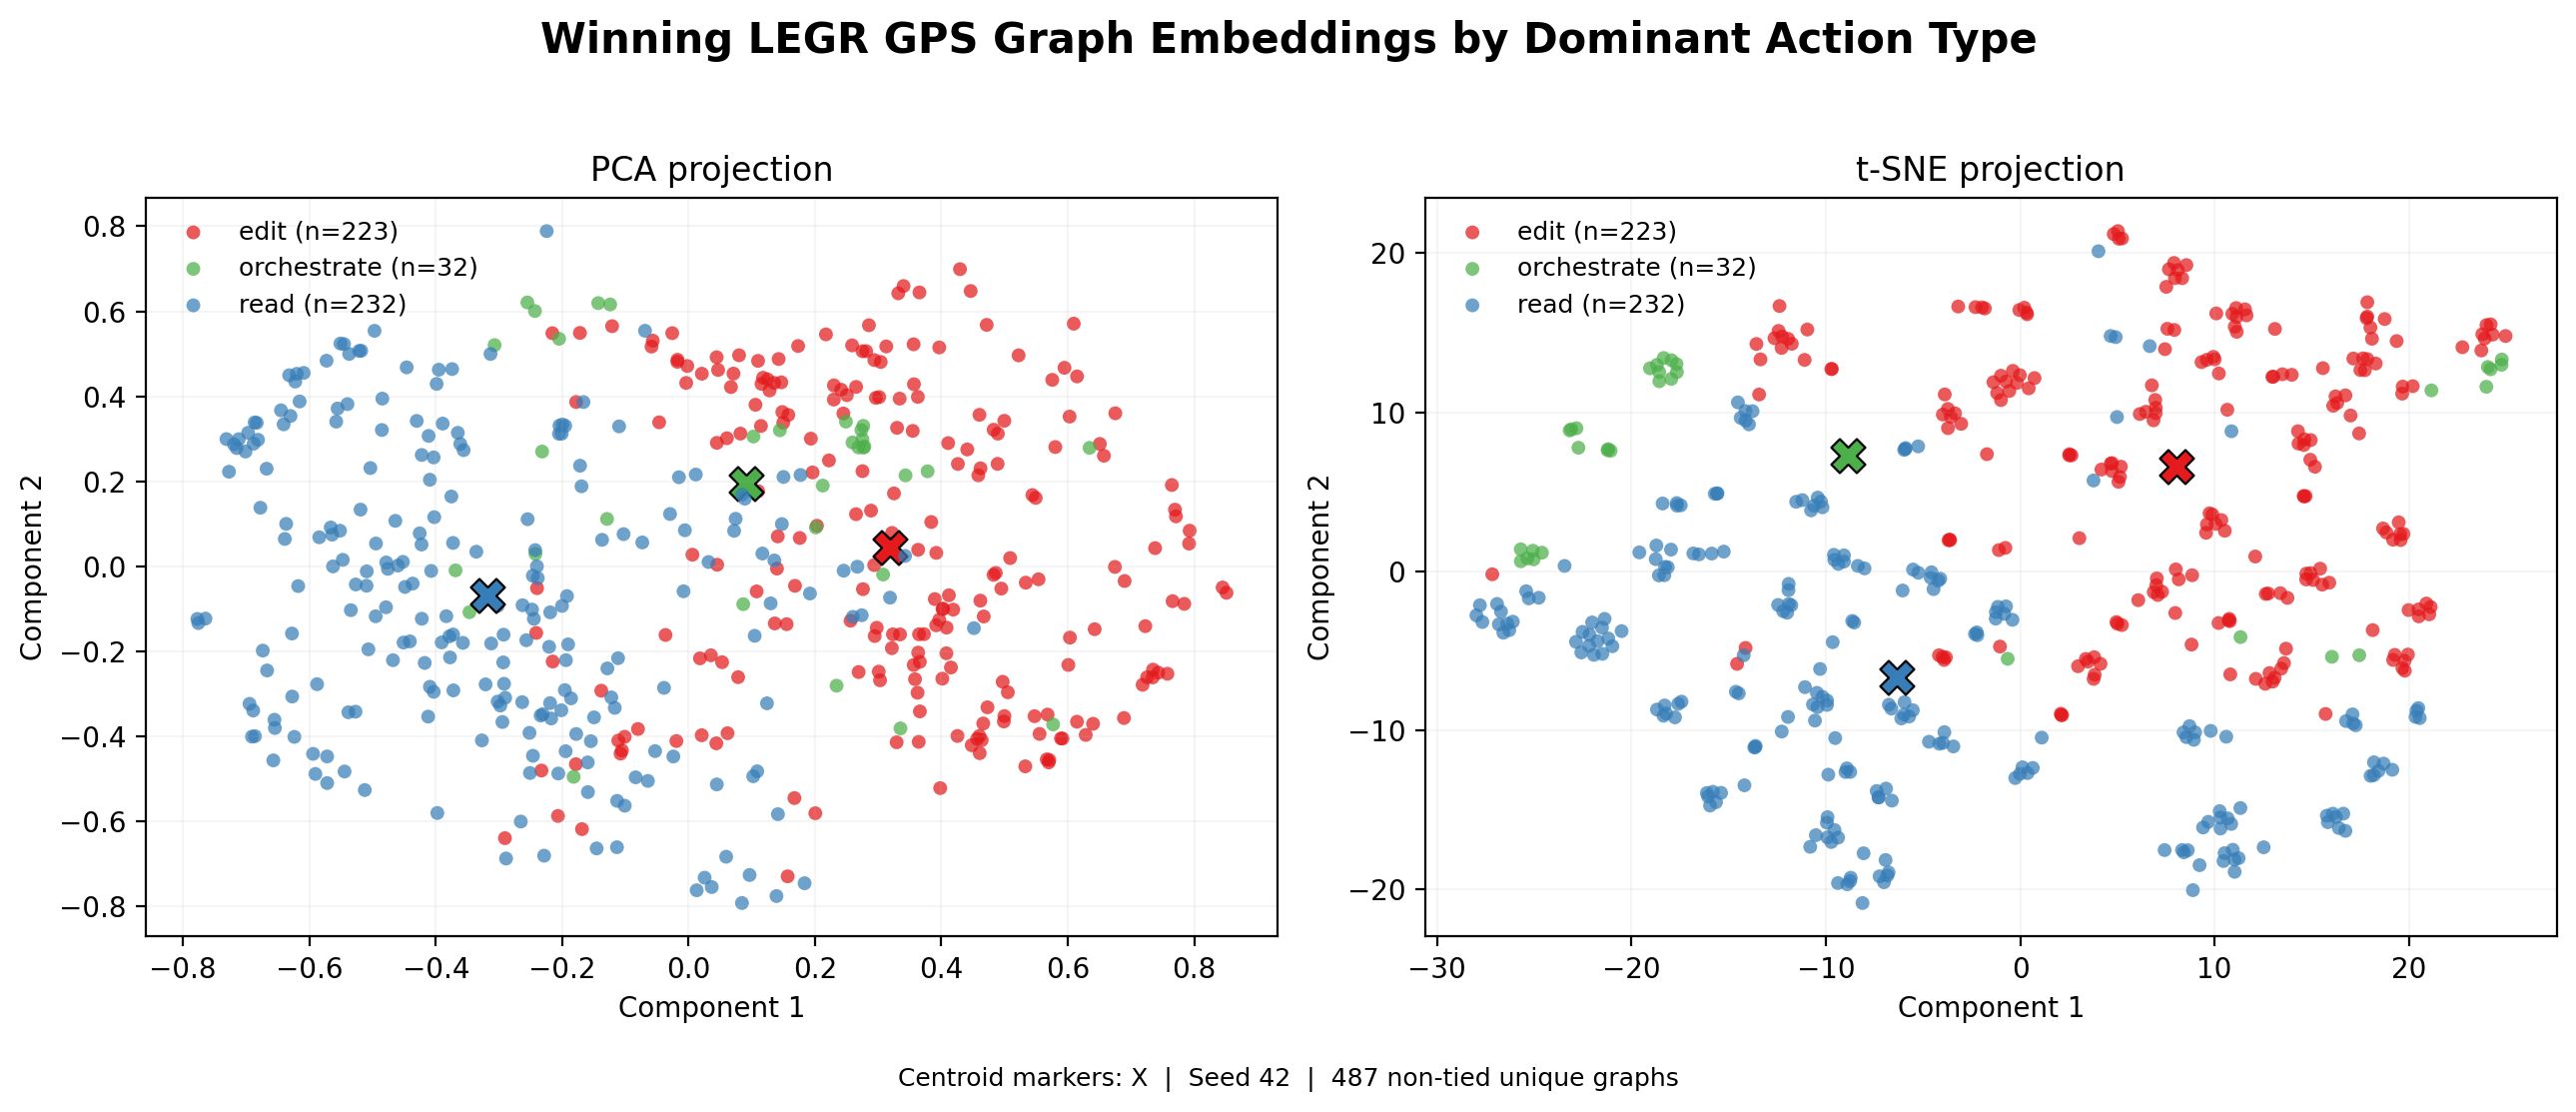
\includegraphics[width=\linewidth]{winning_gps_clusters_scatter.png}
\caption{PCA and t-SNE projections of 487 non-tied graphs from the seed-42 GPS checkpoint, colored by dominant registry action. Crosses mark centroids. Projections are illustrative only; statistical tests use cosine distance in the original 256-dimensional space. The population includes training and evaluation graphs.}
\label{fig:clusters}
\end{figure}

\begin{table}[t]
\caption{Functional organization in the original embedding space.  Permutation $p\leq0.001$ for every listed silhouette, macro-F1, and distance-gap statistic.}
\label{tab:clusters}
\centering
\small
\begin{tabular}{lrrrr}
\toprule
Embedding & Sil. & 5-NN macro-F1 & Purity & Dist. gap \\
\midrule
GPS adapter & \textbf{.1550} & \textbf{.9462} & \textbf{.8931} & \textbf{.2304} \\
V3 graph & .0873 & .9291 & .8868 & .1888 \\
\sbert{} document & .1163 & .9359 & .8763 & .1619 \\
\bottomrule
\end{tabular}
\end{table}

The GPS macro-F1 bootstrap interval is $[0.9102,0.9735]$, far above three-class chance.
Class-specific neighborhood purity is 0.9466 for read, 0.9390 for edit, and 0.7938 for orchestrate.
This corroborates the limited claim that action-function information is present in graph embeddings.
It does not show that the information emerges independently of tool names, causes retrieval gains, or generalizes to unseen tools: labels are derived from tool identities available to every encoder, and the audit includes training graphs.

\section{Discussion}

\paragraph{What the benchmark measures.}
The contrast between 0.9267 compact and 0.2133 twin-filled Recall@1 illustrates why a high retrieval score is not automatically evidence of graph reasoning.
Compact galleries remain useful for semantic routing, but claims about edge structure require controlled alternatives sharing the same tools.

\paragraph{Why hard factorization helps.}
The two experts have complementary error profiles.
\sbert{} identifies the correct tool set strongly; V3 produces graph-dependent representations and slightly improves twin discrimination.
Soft fusion forces one learned score to negotiate both responsibilities and can change the selected tool set.
The hard feasible-set construction in Eq.~\ref{eq:stage2} provides an invariant: the structural module cannot lower tool-set F1.
This is useful even when its structural gain is modest.

\paragraph{Why the remaining gap is large.}
The two-stage mean Recall@1 of 0.2756 remains far from reliable workflow retrieval.
The reranker learns on training-family same-tool-set pairs, while the final gold graphs come from held-out diamond and asymmetric fork--join families.
Moreover, Stage~1 is an error ceiling: if \sbert{} selects the wrong tool set, Stage~2 cannot recover.
Future work should train structure-specific encoders with topology-balanced twin groups and evaluate on a fresh, uninspected held-out corpus.

\paragraph{Functional versus semantic structure.}
Functional action labels and graph topology are related but distinct.
The cluster audit shows that operational categories organize all three embedding spaces, most strongly for GPS under the measured diagnostics.
The twin benchmark then asks whether embeddings also resolve partial order after tool identity is controlled.
Together, these results suggest that useful plan representations must retain semantic function while allocating explicit capacity to dependency relations.

\section{Limitations and Broader Impact}

The evaluation covers 15, 30, and 45 tools but remains within one synthetic benchmark design, two held-out topology families, and machine-generated queries.
Six paraphrases per graph increase query coverage but not the number of independent graph units; clustered intervals correctly expose the resulting uncertainty.
The 15-tool two-stage result is post-hoc because its evaluation gallery had already been inspected; the 30/45 architecture was fixed beforehand, but these tiers are not substitutes for a new independently generated benchmark.
Each tier has one seed-42 V3 checkpoint, so the three-seed variation for \method{} covers the residual reranker, not the expensive base encoders.
Only MiniLM was available for the architecture search, so conclusions do not compare modern embedding backbones.
Latency for the two-stage composition has not yet been rebenchmarked under the locked synchronized protocol; we therefore make no new efficiency claim for it.

The candidate corpus bounds what retrieval can output.
Offline validation can reduce syntactic and cyclic failures, but an incorrect retrieved workflow may still invoke state-changing tools.
Deployed systems should retain permission checks, argument validation, dry-run modes, and human confirmation for consequential operations.
Functional categories may help organize risk, but they are not a substitute for capability security.

\section{Conclusion}

Execution-graph retrieval should be evaluated beyond tool-set recognition.
When every query is paired with same-tool-set structural alternatives, previously strong dense and graph encoders fall sharply, and a sophisticated soft-fusion GPS architecture selected on an easy gallery fails to transfer.
The resulting diagnosis leads to a simpler architecture: use \sbert{} for the semantic decision it performs well, and a V3-initialized pair scorer only for the structural choice it can improve.
This two-stage design increases Recall@1 over \sbert{} from 0.2133 to 0.2756 at 15 tools, 0.1762 to 0.3246 at 30 tools, and 0.1700 to 0.3611 at 45 tools, without changing tool-set F1 or any data.
The 30/45 clustered intervals exclude zero, while the 15-tool interval and its post-hoc status preclude a universal superiority claim.
Standalone V3's 0.4183 Recall@1 at 45 tools further shows that hard semantic preservation and maximum exact-plan recall are distinct operating points.

\section*{Acknowledgments}
Omitted for anonymous review.

\bibliographystyle{plainnat}
\bibliography{references,references_new}

\appendix

\section{Reproducibility Details}

\subsection{Immutable-data guarantee}

No Campaign-v4 CSV, split assignment, existing model source, or existing checkpoint was modified.
New work was isolated in a separate experiment package and artifact directory.
Targets such as tool membership, relation class, dominant action category, and same-tool-set membership were derived transiently from existing \texttt{tools} and \texttt{edges} fields.
Before/after SHA-256 manifests for the final evaluation, functional audit, and two-stage run report zero changed, missing, or added protected files.

\subsection{Two-stage training details}

Both \sbert{} and V3 are loaded read-only from a seed-42 checkpoint at the corresponding tier.
The 15-tool V3 checkpoint pre-existed this study; new 30- and 45-tool V3 checkpoints use the identical architecture and training protocol and are saved under new artifact names.
Candidate and query embeddings are cached.
The pair head has LayerNorm over 1,024 features, a 256-unit linear layer, GELU, dropout, and a scalar output layer.
The output layer is zero initialized.
At 15 tools, seeds 42, 123, and 2026 select reranker epochs 30, 60, and 25.
At 30 tools they select epochs 10, 5, and 5; at 45 tools they select epochs 15, 5, and 15.
The completed reranker/evaluation stages took 38.77, 14.83, and 21.36 seconds at 15, 30, and 45 tools, respectively, excluding base V3 training.

\begin{table}[h]
\caption{Expanded-development performance used for two-stage checkpoint selection.}
\centering
\small
\begin{tabular}{rrrrr}
\toprule
Seed & Epoch & Structural Twin-R@1 & System R@1 & System Twin-R@1 \\
\midrule
42 & 30 & 0.8267 & 0.7585 & 0.7333 \\
123 & 60 & 0.8200 & 0.7551 & 0.7267 \\
2026 & 25 & 0.8267 & 0.7551 & 0.7267 \\
\bottomrule
\end{tabular}
\end{table}

\section{Complete Mathematical Screen}

The first six rows below are cumulative additions, not one-factor removals from the final model.

\begin{table}[h]
\caption{Mathematical objective and batching screen on the original development gallery.}
\centering
\scriptsize
\begin{tabular}{lrrrrr}
\toprule
Variant & R@1 & R@3 & R@5 & Tool-F1 & Toolset R@1 \\
\midrule
Listwise only & .8980 & .9898 & .9932 & .9866 & .9388 \\
$+$ multi-positive & .8912 & .9898 & .9966 & .9837 & .9388 \\
$+$ twin listwise & .8810 & .9898 & 1.0000 & .9764 & .9456 \\
$+$ tool BCE & .8980 & .9898 & 1.0000 & .9857 & .9456 \\
$+$ relation CE & .8912 & .9830 & .9966 & .9837 & .9456 \\
$+$ relation distance & .8912 & .9830 & .9966 & .9837 & .9456 \\
Pairwise margin .1 & .9014 & .9830 & 1.0000 & .9862 & .9456 \\
Pairwise margin .2 & .9014 & .9830 & 1.0000 & .9862 & .9456 \\
Pairwise margin .4 & .8980 & .9830 & 1.0000 & .9857 & .9456 \\
Weights $\times.5$ & .9048 & .9898 & 1.0000 & .9867 & .9456 \\
Weights $\times2$ & .8673 & .9796 & .9898 & .9767 & .9422 \\
Random batches & .8878 & .9932 & .9932 & .9780 & .9490 \\
\bottomrule
\end{tabular}
\end{table}

The intended full research loss was
\begin{equation}
\mathcal L=\mathcal L_{\mathrm{list}}+\mathcal L_{\mathrm{twin}}
+0.5\mathcal L_{\mathrm{tool}}+\mathcal L_{\mathrm{relation}}
+0.1\mathcal L_{\mathrm{multi+}}+0.1\mathcal L_{\mathrm{distance}}.
\end{equation}
The screen shows that this intuitively richer objective is not automatically better than a narrower ranking objective.

\section{Encoder and Readout Screens}

\begin{table}[h]
\caption{Full encoder/structural-input screen. ``PNA-style'' is a directional aggregation variant, not the canonical PNA operator.}
\centering
\scriptsize
\begin{tabular}{lrrrr}
\toprule
Encoder / input & R@1 & Tool-F1 & Toolset R@1 & p95 ms \\
\midrule
V3-style / none & .9048 & .9881 & .9456 & 2.06 \\
V3-style / combined & .9048 & .9867 & .9456 & 1.39 \\
Residual / none & .9048 & .9881 & .9456 & 2.06 \\
Residual / combined & .9048 & .9867 & .9456 & 1.55 \\
Gated / none & .8980 & .9796 & .9490 & 1.76 \\
Gated / combined & .8946 & .9796 & .9456 & 1.38 \\
PNA-style / none & .8946 & .9864 & .9456 & 1.78 \\
PNA-style / combined & .8980 & .9852 & .9490 & 1.49 \\
Graphormer / none & .9116 & .9873 & .9490 & 13.63 \\
Graphormer / combined & .9082 & .9870 & .9490 & 15.54 \\
GPS / none & .9082 & .9873 & .9490 & 14.20 \\
GPS / combined & .9116 & .9878 & .9490 & 13.64 \\
GPS / depth & .9116 & .9878 & .9490 & 15.62 \\
GPS / degree-source-sink & .9150 & .9892 & .9490 & 15.09 \\
GPS / path & .9082 & .9873 & .9490 & 13.43 \\
\bottomrule
\end{tabular}
\end{table}

The labels V3-style and residual map to the same residual local block in the experimental adapter and therefore are not independent architectures.
Total topological-sort rank was excluded from new structural inputs because parallel nodes receive an arbitrary order.
Relation attention instead uses directed path and reachability information.

\begin{table}[h]
\caption{Readout screen on the residual adapter.}
\centering
\small
\begin{tabular}{lrrr}
\toprule
Readout & R@1 & Tool-F1 & Toolset R@1 \\
\midrule
Mean/V3 style & .9082 & .9872 & .9456 \\
Dual attention & .9048 & .9867 & .9456 \\
Virtual attention & .9082 & .9879 & .9456 \\
Set2Set & .8912 & .9829 & .9388 \\
Concatenated statistics & .9082 & .9879 & .9456 \\
\bottomrule
\end{tabular}
\end{table}

\section{Reranker and Optimization Screens}

\begin{table}[h]
\caption{Candidate-aware cross-attention rerankers.}
\centering
\small
\begin{tabular}{rrrrr}
\toprule
Top-$K$ & Layers & R@1 & Tool-F1 & p95 ms \\
\midrule
10 & 1 & .6565 & .8379 & 25.44 \\
10 & 2 & .7279 & .9003 & 36.16 \\
20 & 1 & .6190 & .8371 & 35.33 \\
20 & 2 & .7041 & .9025 & 57.58 \\
40 & 1 & .7857 & .9418 & 58.34 \\
40 & 2 & .5884 & .8318 & 88.03 \\
\bottomrule
\end{tabular}
\end{table}

These rerankers differ from \method{} in two important respects: they rerank an unconstrained semantic top-$K$, and they were selected on the sparse-twin development gallery.
Their failure supports training on explicit same-tool-set pairs and preventing the structural component from changing semantic feasibility.

\begin{table}[h]
\caption{Optimization screen for the GPS route.}
\centering
\small
\begin{tabular}{lrrrr}
\toprule
Setting & R@1 & Tool-F1 & Toolset R@1 & p95 ms \\
\midrule
Backbone frozen & .8571 & .9673 & .9456 & 13.92 \\
Last two layers trainable & .9150 & .9892 & .9490 & 15.88 \\
Full backbone trainable & .9150 & .9892 & .9490 & 24.29 \\
Cosine schedule & .9150 & .9892 & .9490 & 15.87 \\
Plateau schedule & .9082 & .9878 & .9490 & 13.84 \\
EMA & .9082 & .9867 & .9490 & 13.69 \\
SWA & .9082 & .9867 & .9490 & 17.25 \\
Online hard negatives & .9116 & .9887 & .9490 & 15.12 \\
Twin curriculum & .9150 & .9881 & .9524 & 13.63 \\
\bottomrule
\end{tabular}
\end{table}

EMA and SWA were implementation-level screens rather than definitive tests: the EMA path restored the raw state before saving, and SWA replaced the final state without an independent selection criterion.

\section{Historical Campaign-v4 Results}

Early integer-ID graph encoders performed poorly because the graph tower lacked pretrained tool semantics.
At 15 tools and 75 epochs, directed LEGR with GED reached only 0.0800 compact-gallery Recall@1 and 0.3779 tool F1.
Replacing integer IDs with MiniLM tool-name features raised V2 to 0.6200, and sharing the text backbone with a set-plus-directed-GNN readout raised V3 to 0.8267.
SBERT-FT reached 0.9267.
Within V3, removing GED improved Recall@1 from 0.8133 to 0.8267, contradicting any universal claim that GED is necessary.

\begin{table}[h]
\caption{Compact 15-tool checkpoint progression.}
\centering
\small
\begin{tabular}{lrrr}
\toprule
Model & R@1 & Tool-F1 & Mean GED \\
\midrule
Integer directed + GED & .0800 & .3779 & 4.250 \\
V2 tool-name + GED & .6200 & .8241 & 1.690 \\
V3 SetGNN, no GED & .8267 & .9464 & .707 \\
V3 SetGNN + GED & .8133 & .9402 & .763 \\
SBERT-FT, no GED & .9200 & .9781 & .310 \\
SBERT-FT + GED & .9267 & .9811 & .290 \\
\bottomrule
\end{tabular}
\end{table}

\section{Legacy Single-Tool Functional Routing Pilot}

The original manuscript reported a zero-shot single-tool routing pilot comparing topic and functional hierarchies.
We retain it only as historical appendix evidence because the raw prompts, responses, exact model identifiers, and parser artifacts were not recovered in the present audit.
Moreover, the functional hierarchy uses three top-level branches, creating a branching-factor confound that requires a matched control before causal claims about label semantics.

\begin{table}[h]
\caption{Legacy pilot accuracy (\%).  This table is not part of the Campaign-v4 model-search manifest and is not a central claim.}
\centering
\small
\begin{tabular}{llrrrr}
\toprule
Router & Categorization & Standard & Lexical & Confusable & Paraphrase \\
\midrule
GPT-OSS & Topic & 78.3 & 68.1 & 62.7 & 78.0 \\
GPT-OSS & Functional & 93.3 & 75.6 & 68.0 & 90.6 \\
Llama 3.2 & Topic & 70.0 & 43.3 & 43.3 & 64.9 \\
Llama 3.2 & Functional & 83.8 & 61.8 & 55.3 & 79.8 \\
\bottomrule
\end{tabular}
\end{table}

The largest reported difference is 18.5 percentage points for Llama under lexical stress.
This observation motivated the functional embedding audit in Section~7, but that audit is not a substitute replication: graph labels derive from the registry, whereas the legacy study evaluates an LLM router.

\section{Generative Baselines and Protocol Non-equivalence}

Corrected v3 runs used the dynamic Campaign-v4 vocabulary and a 1,024-token generation cap.
\begin{table}[h]
\caption{Full corrected DAG-generation diagnostics. Valid counts structurally valid parsed DAGs.}
\centering
\scriptsize
\begin{tabular}{lrrrrrrr}
\toprule
Model & Tools & Parse fail. & Cyclic & Valid & Tool-F1 & EM & GED \\
\midrule
GPT-OSS 120B & 15 & 0 & 0 & 50 & .9450 & .76 & .44 \\
             & 30 & 0 & 0 & 50 & .9517 & .80 & .62 \\
             & 45 & 0 & 0 & 50 & .9486 & .76 & .80 \\
Llama 3.2 3B & 15 & 0 & 6 & 44 & .7911 & .08 & 6.11 \\
              & 30 & 2 & 4 & 44 & .7769 & .06 & 4.80 \\
              & 45 & 5 & 2 & 43 & .6844 & .04 & 4.58 \\
\bottomrule
\end{tabular}
\end{table}
These models emit one potentially novel plan rather than ranking a fixed gallery, so exact match must not be placed in the same statistical column as retrieval Recall@1.

\section{Artifact and Evaluation Checklist}

For reproducibility, a release should include:
\begin{itemize}[leftmargin=*]
    \item all resolved configurations, seeds, epoch histories, checkpoints, and score matrices;
    \item canonical graph hashes and before/after protected-file manifests;
    \item the fixed gallery permutation and tie tolerance;
    \item per-query predictions sufficient to recompute Recall@$k$, MRR, tool F1, twin metrics, GED, and clustered bootstrap intervals;
    \item the functional label CSV, original 256-dimensional embeddings, projection coordinates, and permutation/bootstrap outputs;
    \item hardware, software versions, synchronized latency warm-up/trial counts, and candidate-cache policy.
\end{itemize}

\section{Use of Large Language Models}

GPT-4o was used to generate the six natural-language query variants associated with each Campaign-v4 graph; the generation ledger records 2,781 successful calls, 1,447,171 prompt tokens, 1,102,497 completion tokens, and zero failed calls.
LLM-assisted coding tools were used during implementation, debugging, experiment orchestration, and manuscript drafting.
All reported numerical claims were read from saved experiment artifacts or recomputed by deterministic evaluation code; protected datasets and checkpoints were hash checked before and after the work.
Authors remain responsible for the experimental design, source verification, interpretation, and final text.

\end{document}
